\documentclass{article}
\usepackage{amssymb}
\usepackage{amsmath}
\usepackage{geometry}
\usepackage{graphicx}
\usepackage{float}

\geometry
{
a4paper,
total={170mm,257mm},
left=20mm,
top=20mm,
}

\newcommand{\s}{\text{ }}

\title{Design for a P System Program - A P System Editor and Simulator}
\date{\today}
\author{Ren Tristan A. de la Cruz: SN\#2008-35070}

\begin{document}
\maketitle

% ================================================================================================ %

\section{Preliminaries}

% ================================================================================================ %


\subsection{Membrane Computing}\label{s-memcom}

% ================================================================================================ %

\textit{Membrane computing} is a field of theoretical computer science that studies different models
of computation known as \textit{P systems}. The term `\textit{P systems}' refers to a family of
models of computation which are inspired by biological processes. P system models use abstractions
of biological processes as computational operations. For example, different types of rules
(operations) used by most P system variants are abstractions of processes like \textit{chemical
reaction} and \textit{ion transport} that occur inside biological cells. Most P system variants use 
\textit{object symbols} as the objects of computation. One can think of these object symbols as 
abstraction of physical \textit{molecules} or \textit{ions}. P systems store \textit{multisets} of
these object symbols inside regions enclosed by \textit{membranes}. A P system has a collection of
these membranes with multisets of objects symbols inside. The membranes can be `connected' to each
other to form a \textit{membrane structure}.

% ================================================================================================ %

\subsection{Components of a P System}\label{s-psystem}

Currently, there are tens, if not hundreds, of P system variants. The following sections describe 
the components that are common to most (if not all) P system variants.

\subsubsection{Membrane Structure}\label{s-membrane}

A P system has set of membranes that can be connected to each other. These connected membranes form
a \textit{membrane structure}. Early P systems are described as \textit{cell-like} since their 
membrane structures are inspired by nested membranes inside a cell. Figure \ref{fig:cell-like} shows 
an example of a cell-like membrane structure.

\begin{figure}[H]
\begin{center}
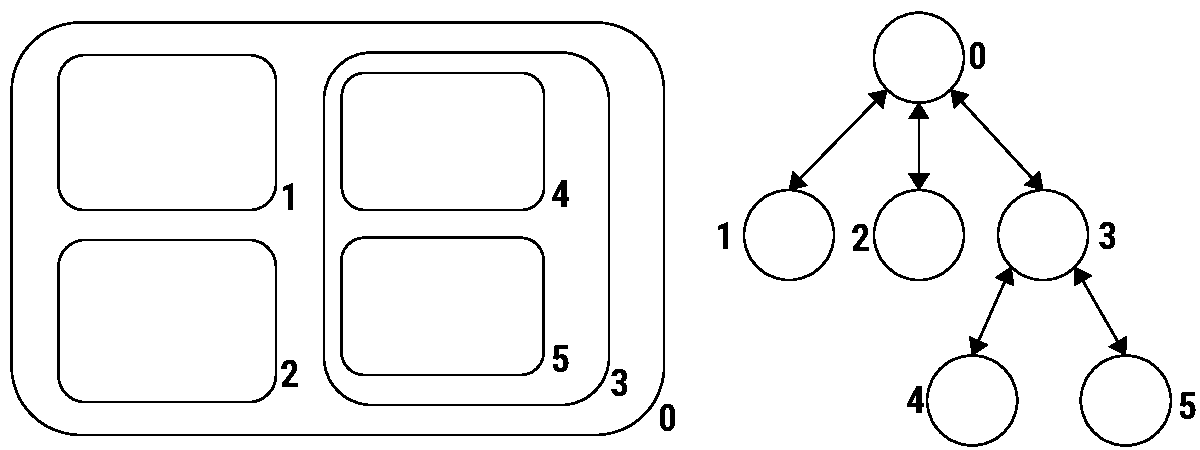
\includegraphics[scale=0.60]{figures/zzz-cell-like-structure.pdf}
\caption{Cell-like Membrane Structure}
\label{fig:cell-like}
\end{center}
\end{figure}

In Figure \ref{fig:cell-like} you can see two representations of a 6-membrane cell-like membrane 
structure. The left diagram shows the nesting of the membranes while right diagram shows the tree 
topology of the membranes. The outer most membrane, membrane 0, is the root node of the tree while 
membranes that do not contain internal membranes (membranes 1,2,4,5) are the leaf nodes of the tree.

Other P system variants use the more general graph membrane structure. P systems described as
\textit{tissue-like} or \textit{neural-like} use graph membrane structures. In \textit{tissue-like}
P systems, the membranes are called \textit{cells} and the connected cells form a `\textit{tissue}'. 
In \textit{neural-like} P systems, the membranes are called \textit{neurons} and the connected 
neurons form a \textit{neural network}. Figure \ref{fig:graph-topology} shows an example of a graph
membrane structure with 7 membranes.

\begin{figure}[H]
\begin{center}
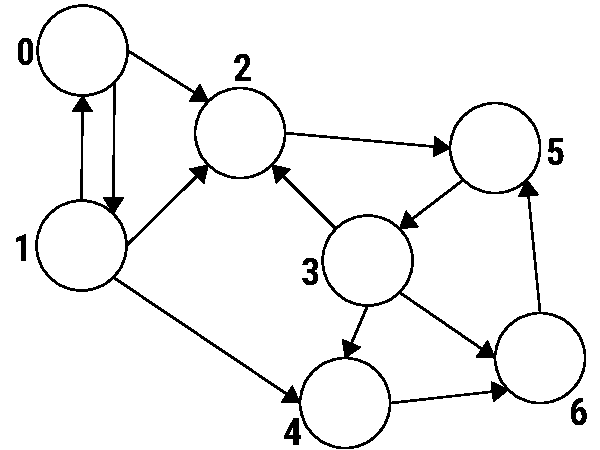
\includegraphics[scale=0.60]{figures/zzz-graph-topology.pdf}
\caption{Graph Membrane Structure}
\label{fig:graph-topology}
\end{center}
\end{figure}

% ================================================================================================ %

\subsubsection{Multisets of Object Symbols}\label{s-multiset}

As mentioned in Section \ref{s-memcom}, the objects of computation in P systems are abstract
object symbols. Any P system has a fixed set of object symbols or an \textit{alphabet}. We denote 
this alphabet of object symbols as $V$. A multiset over alphabet $V$ is simply a set of object 
symbols from $V$ in which multiple instances of the same object symbols are allowed. For example, 
given the alphabet $V = \{a,b,c,d\}$, the following are some multisets over $V$:

\begin{itemize}
\item $\{a,a,b\}$
\item $\{a,a,b,c,c,d\}$
\item $\{c,d,d\}$
\item $\{a,c,c,c,d,d\}$
\item $\{a,a,b,b,b,c,c,c,c,d,d,d,d,d\}$
\end{itemize}

Multisets can be written as strings. For example:

\begin{itemize}
\item $\{a,a,b\} = aab = a^2b$
\item $\{a,a,b,c,c,d\} = aabccd = a^2bc^2d$
\item $\{c,d,d\} = cdd = cd^2$
\item $\{a,c,c,c,d,d\} = acccdd = ac^3d^2$
\item $\{a,a,b,b,b,c,c,c,c,d,d,d,d,d\}= aabbbccccddddd=a^2b^3c^4d^5$
\end{itemize}

In a P system, regions enclosed by membranes store multisets of object symbols. Figure 
\ref{fig:multisets-on-membranes} shows two examples of membrane structures (cell-like and graph) 
with multisets of symbols in the  regions.

\begin{figure}[H]
\begin{center}
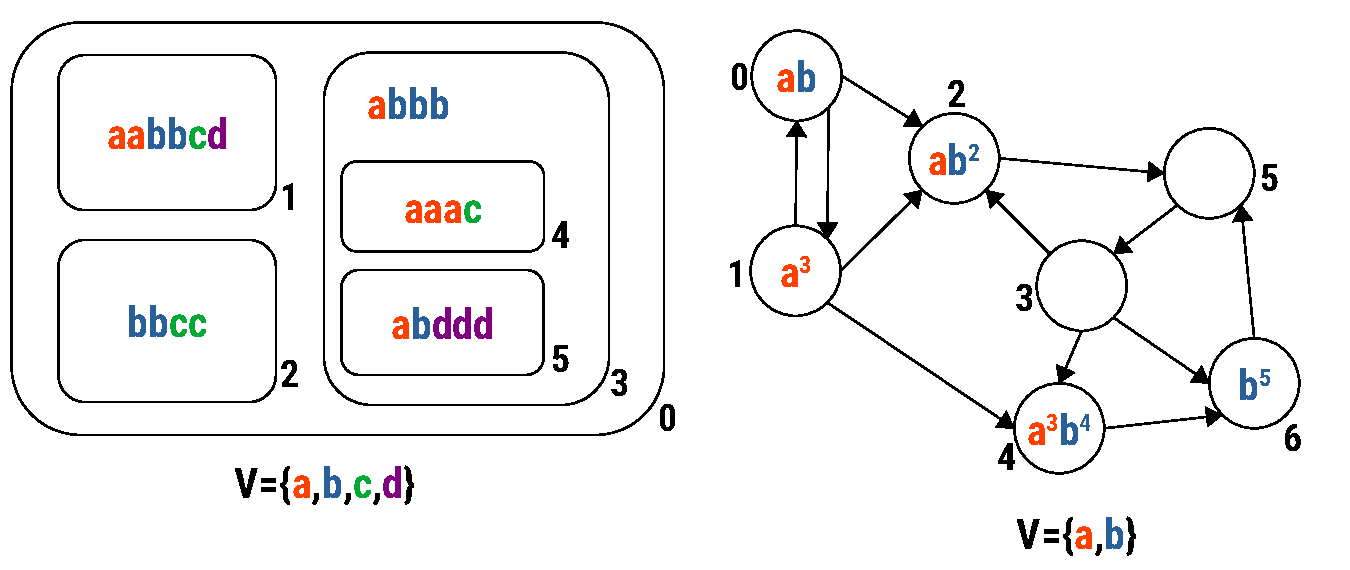
\includegraphics[scale=0.55]{figures/zzz-multisets-on-membranes.pdf}
\caption{Multisets in Membrane Structures}
\label{fig:multisets-on-membranes}
\end{center}
\end{figure}

The left diagram in Figure \ref{fig:multisets-on-membranes} shows the membrane structure from Figure
\ref{fig:cell-like} with multisets over alphabet $V=\{a,b,c,d\}$. Membrane 0 is empty (or contains 
the empty multiset). Membrane 1 contains the multiset $aabbcd$. Membrane 2 contains the multiset
$bbcc$. Membrane 3 contains the multiset $abbb$, etc. The right digram in Figure 
\ref{fig:multisets-on-membranes} shows the membrane structure from Figure \ref{fig:graph-topology} 
with multisets over alphabet $V=\{a,b\}$. Cell 0 contains the multiset $ab$. Cell 1 contains the 
multiset $a^3$. Cell 2 contains the multiset $ab^2$. Cell 3 is empty, etc. 


% ================================================================================================ %

\subsubsection{Rules of Different Types}\label{s-rule}

A P system uses a set of rules to perform computation. Different P system variants use different
types of rules. In general, a rule transforms the multisets inside the membranes and/or transforms
the membrane structure itself. Static structure P systems only use rules that primarily
transform the multisets inside the membranes and do not change the structure of the system. Dynamic
structure P systems have rules that can add new membranes, delete existing membranes, and change the
connections between membranes.

Rules for transforming multisets inside the membranes are based on \textit{multiset rewriting 
rules}. A \textit{multiset rewriting rule} is written as $M \rightarrow M'$ where $M$ and $M'$ are 
both multisets over the same alphabet. The rule rewrites the multiset $M$ to the multiset $M'$.

For example: Alphabet is $V = \{a,b,c,d\}$

\begin{itemize}

\item \texttt{Rule 1}: $a^2b^2 \rightarrow cd$
\begin{itemize}
\item Applying \texttt{Rule 1} once to multiset $a^4b^5c^3d^2$ will transform it to $a^2b^3c^4d^3$.
\item Applying \texttt{Rule 1} twice to multiset $a^4b^5c^3d^2$ will transform it to $bc^5d^4$.
\end{itemize}

\item \texttt{Rule 2}: $ad \rightarrow ab^2c^3$
\begin{itemize}
\item Applying \texttt{Rule 2} once to multiset $a^4b^5c^3d^2$ will transform it to $a^4b^7c^6d$.
\item Applying \texttt{Rule 2} twice to multiset $a^4b^5c^3d^2$ will transform it to $a^4b^9c^9$.
\end{itemize}

\end{itemize}

The first P system, known as \textit{transition P system}, is a cell-like P system that uses 
modified multiset rewriting rules. Rules in transition P systems are multiset rewriting rules that
use the membrane structures of the systems. A rule is associated with the region enclosed by a 
specific membrane. A rule will `consume' a multiset of object symbols in its region then it can
produce multisets of object symbols in the same (\textit{here}) region, in the region outside 
(\textit{out}) its membrane, and/or in the regions enclosed by membranes inside (\textit{in}) the
rule's own membrane. Figure \ref{fig:trans-rule} shows an example of a rule being applied.

\begin{figure}[H]
\begin{center}
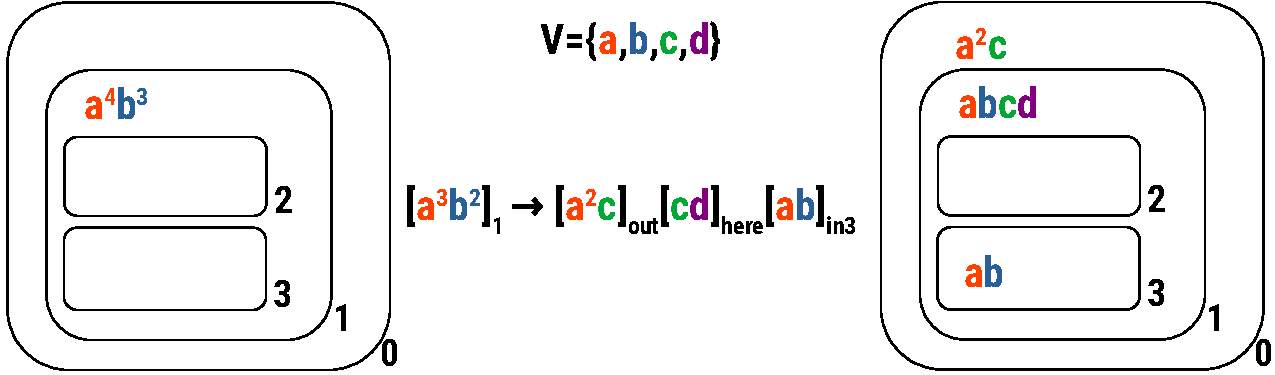
\includegraphics[scale=0.55]{figures/zzz-transition-rule.pdf}
\caption{Application of Transition Rule $[a^3b^2]_1 \rightarrow [a^2c]_{out}[cd]_{here}[ab]_{in_3}$}
\label{fig:trans-rule}
\end{center}
\end{figure}

The left diagram on Figure \ref{fig:trans-rule} shows the \textit{configuration} of the system
before rule application. Membrane 1 contains the multiset $a^4b^3$ while the other membranes are 
empty. The rule $[a^3b^2]_1 \rightarrow [a^2c]_{out}[cd]_{here}[ab]_{in_3}$ is associated with the
region  enclosed by membrane 1. The rule consumes $a^3b^2$ from membrane 1, produces $a^2c$ outside 
membrane 1 (in membrane 0), and produces $ab$ inside membrane 3. The right diagram on Figure 
\ref{fig:trans-rule} shows the configuration of the system after the rule is applied.

It can also be specified in a rule in a transition P system that the membrane associated with the 
rule be \textit{dissolved} after the rule was applied. Figure \ref{fig:trans-rule2} shows how a rule
can \textit{dissolve} a membrane. Rule $[a^2b^2]_1 \rightarrow [ab]_{in_2}[cd]_{in_3}\delta$ 
consumes multiset $a^2b^2$ from membrane 1, produces multiset $ab$ in membrane $2$, produces 
multiset $cd$ in membrane 3, and \textit{dissolves} membrane 1 (this is specified by $\delta$ at the
end of the rule). The remaining multiset in membrane 1 will go to its parent membrane, membrane 0.

\begin{figure}[H]
\begin{center}
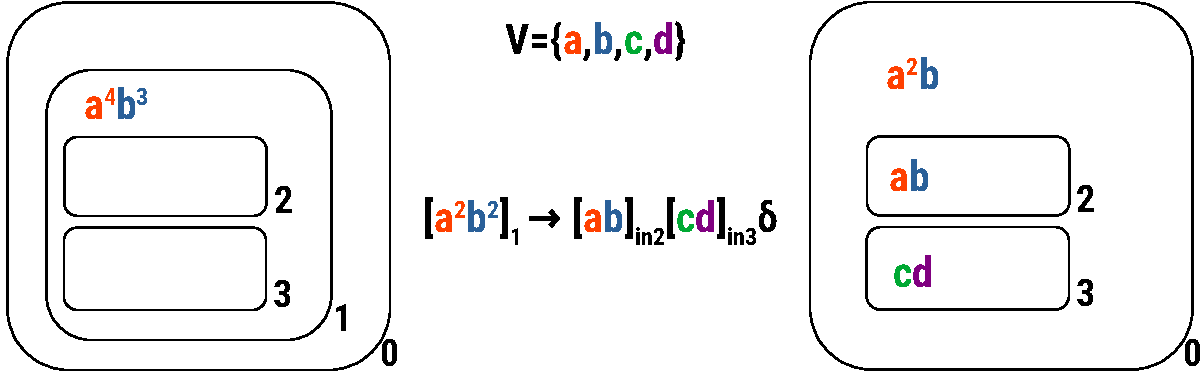
\includegraphics[scale=0.55]{figures/zzz-transition-rule2.pdf}
\caption{Application of Transition Rule $[a^2b^2]_1 \rightarrow [ab]_{in_2}[cd]_{in_3}\delta$}
\label{fig:trans-rule2}
\end{center}
\end{figure}

\textit{Tissue P systems}' rules are very similar to rules in transition P systems. The difference 
is that tissue P systems' membrane structures form graphs that do not have directionality or
orientation unlike the tree membrane structures of transition P systems. When you are in the node
of a tree in the membrane structure of a transition P system, the rule can send produced multisets
\textit{out} in the direction of the parent node, in the same node (\textit{here}), or in the
direction of the children nodes (\textit{in}). In tissue P systems, a rule can send produced 
multisets in the same node (\textit{here}) or to the adjacent nodes (\textit{out}). Aside from this
rule convention, rules in tissue P systems also have multiple different semantic meanings.

\begin{figure}[H]
\begin{center}
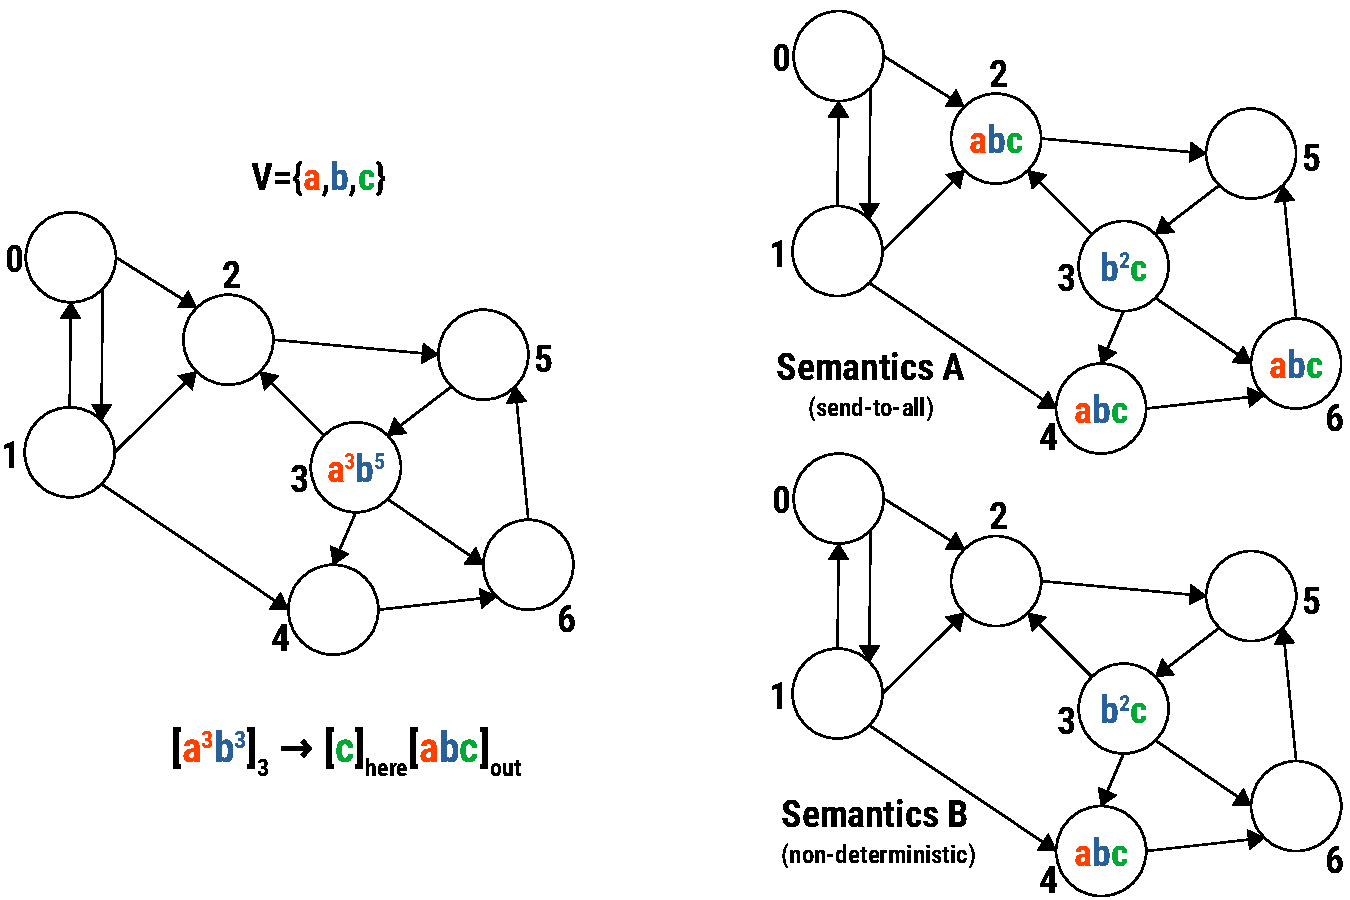
\includegraphics[scale=0.55]{figures/zzz-tissue-rule.pdf}
\caption{Application of Tissue P system Rule $[a^3b^3]_3 \rightarrow [c]_{here}[abc]_{out}$}
\label{fig:tissue-rule}
\end{center}
\end{figure}

Figure \ref{fig:tissue-rule} shows two interpretations (Semantics A and B) for the rule 
$[a^3b^3]_3 \rightarrow [c]_{here}[abc]_{out}$. For semantics A, the rule consumes multiset 
$a^3b^3$ from cell 3, produces multiset $c$ in cell 3, and sends multiset $abc$ to all adjacent
cells (cells 2,4,6). For semantics B, the rule consumes multiset $a^3b^3$ from cell 3, produces
multiset $c$ in cell 3, and \textit{nondeterministically} sends multiset $abc$ to one of the
cells adjacent to cell 3 (either cell 2,4, or 6).

P systems \textit{with active membranes} introduced a type of rule that allows creation of new
membranes. Figure \ref{fig:active-mem-rule} shows a rule of this type. The rule $[a]_y \rightarrow
[b]_y[c]_y$ in Figure \ref{fig:active-mem-rule} has a very similar syntax to previous rules but its
semantics is different. The rule consumes the object symbol $a$ in membrane labeled $y$. The rule 
will then duplicate the membrane copying all the remaining object symbols to both membrane copies.
Both membrane copies are also labeled $y$. In this P system variant, membrane labels are not
membrane ids so multiple membranes can have the same label. In one of the copies, object symbol 
$b$ is produce while in the other copy object symbol $c$ is produced. Figure
\ref{fig:active-mem-rule} shows the rule being applied twice in two steps.

\begin{figure}[H]
\begin{center}
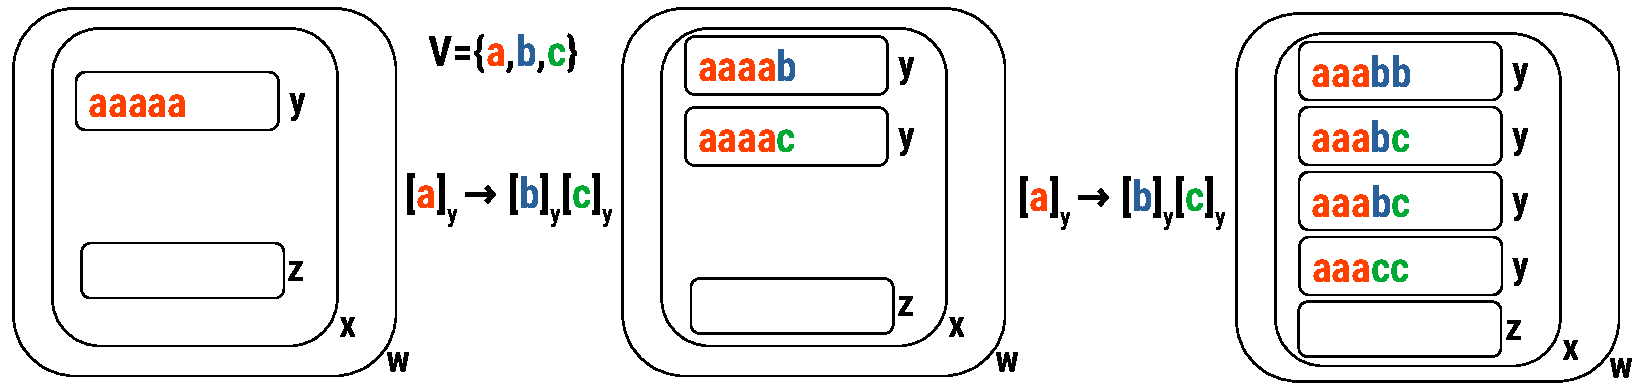
\includegraphics[scale=0.55]{figures/zzz-active-mem-rule.pdf}
\caption{Application of the Active Membrane Rule $[a]_y \rightarrow [b]_y[c]_y$}
\label{fig:active-mem-rule}
\end{center}
\end{figure}

The types of rules described above form a small set of samples of all possible types of rules. A 
large portion of the other types of rules that are not discussed are variations of the rules 
above. Some of them may have a slightly different semantics to the rules above.

% ================================================================================================ %

\subsubsection{P System Derivation Modes}\label{s-derivation}

P systems are parallel computing models. A P system can apply multiple rules at the same time.
Different P systems can have different conventions that say which combinations of rules can be 
applied at the same time. This convention is known as the \textit{derivation mode} of the system.
A common derivation mode is called \textit{maximally parallel} derivation mode. In maximally
parallel mode, the system will apply a combination of rules such that you can no longer add 
instances of rules to this \textit{maximal} combination of rules. For example, you have:

\begin{itemize}
\item \texttt{Rule 1:} $[ab]_1 \rightarrow [xy]_{here}$
\item \texttt{Rule 2:} $[b^2]_1 \rightarrow [xyz]_{here}$ 
\end{itemize}

\texttt{Rule 1} consumes $ab$ from membrane 1 while \texttt{Rule 2} consumes $b^2$
from membrane 1. If membrane 1 contains the multiset $a^3b^6$, one maximal combination of rules is
$3 \times$\texttt{Rule 1} + \texttt{Rule 2}. This combination will consume the multiset $a^3b^5$.
With the multiset $b$ remaining no additional rules can be added to the combination making the
combination maximal. Another maximal combination of rules is $3\times$\texttt{Rule 2}. This
combination will consume the multiset $b^6$. With the multiset $a^3$ remaining no additional rules
can be added. Another maximal combination is $2\times$\texttt{(Rule 1 + Rule 2)} consuming the
multiset $a^2b^6$. In maximally parallel mode, only a maximal combination of rules can be applied.
For example, the system can not apply the combination with one instance of \texttt{Rule 1}, if the
system can still apply additional rules then it will add these rules to the combination. In this
mode, the system \textit{maximizes} the rules it can apply.

\textit{Minimally parallel} mode is often used in \textit{neural-like} P system variants. In the
minimally parallel mode, at most one applicable rule is applied per membrane. The `parallel' part is
that multiple membranes can apply a rule at the same time. The `minimal' part is that at most one
rule can be applied per membrane.

There are other derivations modes. Some P system variants have the same rule types and membrane
structure but only differ in the derivation modes they use.

% ================================================================================================ %
 
\subsection{Purpose of a User-friendly General P Systems Viewer and Simulator}\label{s-purpose}

Manually designing (using pen and paper) a P system is easy for smaller systems (with fewer than 20
membranes). It gets increasing difficult the larger the system is. You have to keep track of the
multisets of object symbols and the rule set per membrane and the connections between the membranes.
Manually simulating P systems is much more difficult than designing one even for smaller systems 
because the components of the system work in parallel (membranes applying rules at the same time). 
Additionally, non-deterministic systems are much more difficult to simulate manually since you have
to keep track of branching computations.

\textit{P-lingua} is well-known P system simulator but it is not particularly user-friendly and its
support for P system variants is limited to the few popular variants. It is a command-line based
simulator and has no built-in P system visualizer. It gives the simulation as text. When creating a
system for the P-lingua simulator, the user has to explicitly type out the system definition in a 
file.

The purpose of a user-friendly general P system simulator and viewer program is to simplify the 
process of designing and simulating P systems. The program should help the users design P systems 
by providing a user-friendly/intuitive interface that they can use to create and modify P systems.
The program should also be able to perform simulation of the system. Additionally, the program 
should be general enough to accommodate most P system variants.

% ================================================================================================ %


\section{Design of the P System Program}\label{s-design}

% ================================================================================================ %

\subsection{P System Program - Editor and Simulator}\label{s-context}

To avoid confusion, we are going to use `program' for the system being designed while the term 
`systems' will refer to P systems (the objects of simulation). The P system program will be a 
standalone P system editor and simulator. The user is the only one interacting with the program. 
There are no external programs that interact with the P system program. The purpose for designing
the program will to be self-contained/standalone is to make it portable and easy to use for 
membrane computing researchers.  

\begin{figure}[H]
\begin{center}
    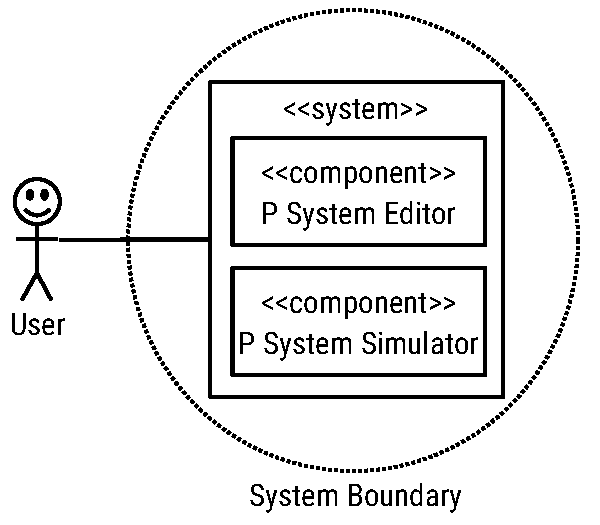
\includegraphics[scale=0.8]{figures/zzz-context-model.pdf}
    \caption{Context for the P System Program}
    \label{fig:context}
\end{center}
\end{figure}

The program will have two main components: the editor and the simulator. The P system editor
contains the user interface to control the program while the P system simulator contains the 
functions needed to generate the P system's computation tree.

% ================================================================================================ %

\subsection{Representing P Systems}\label{s-represent}

We have already described components of a P system in Section \ref{s-psystem}. In this section, we
construct different classes to represent the components of the P system. We also show how these
components (and classes) are related to each other.

\begin{enumerate}

\item \texttt{Membrane} class represents membranes in the P system (see Section 
\ref{s-multiset}). A membrane has three components, the membrane's \textit{id}, the membrane's
\textit{label}, and the membrane's \textit{content} which is a multiset over a given alphabet. The
\texttt{Membrane} class has \texttt{id} (integer), \texttt{label} (string), and \texttt{content}
(multiset) attributes and the additional \texttt{coordinate} (pair of integers) attribute.

\begin{figure}[H]
\begin{center}
    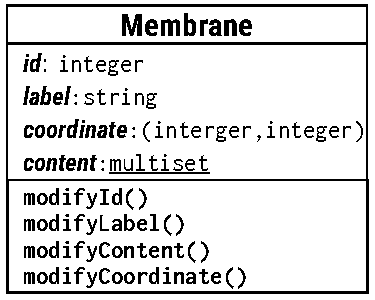
\includegraphics[scale=0.8]{figures/zzz-membrane.pdf}
    \caption{Membrane Class}
    \label{fig:membrane}
\end{center}
\end{figure}

The \texttt{id} attribute is for identifying the membrane. The \texttt{label} attribute is a string
label of the membrane. The \texttt{content} attribute is a multiset type. If we are using a multiset
over an alphabet of size $n$, then a multiset is simply an array of integers of size $n$. For 
example, for an alphabet $V=\{a,b,c\}$, a multiset over $V$ is an array of (non-negative) integers 
of size $3$. The multiset \texttt{[3,2,0]} refers to the multiset $a^3b^2c^0$.

The \texttt{coordinate} attribute will be used when visualizing the membrane. The membrane will be
drawn in 2-dimensional space so a 2D coordinate is needed to specify a membrane's location.

The four methods of the class, \texttt{modifyId(), modifyLabel(), modifyContent(), 
modifyCoordinate()}, are used to modify the values of the corresponding attributes.

% ================================================================================================ %

\item \texttt{Configuration} class represents the \textit{configuration} (or state) of the P system
(see Sections \ref{s-membrane} and \ref{s-multiset}). The \textit{configuration} of a P system is 
its network of membranes. The \texttt{configuration} class has the following attributes: 
\texttt{id} (integer), \texttt{time} (integer), \texttt{membranes} (set of \texttt{membranes}), 
\texttt{connections} (set of \texttt{membrane} id pairs).

\begin{figure}[H]
\begin{center}
    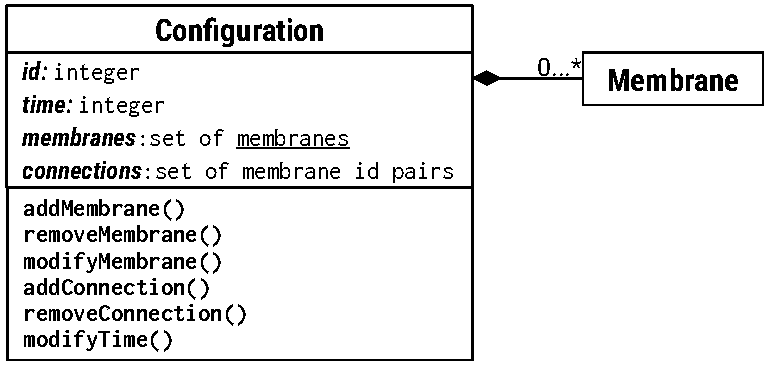
\includegraphics[scale=0.8]{figures/zzz-configuration.pdf}
    \caption{Configuration Class}
    \label{fig:configuration}
\end{center}
\end{figure}

The \texttt{id} attribute is for configuration identification. The \texttt{time} attribute is the
time step when the P system had the configuration. The initial configuration of the P system has the
\texttt{time} attribute set to \texttt{0}. The next configurations will have the \texttt{time} 
attribute set to \texttt{1}. The \texttt{membranes} attribute is the set of \texttt{membrane} 
objects while the \texttt{connections} attribute is the set of pairs of \texttt{membrane} object 
\texttt{ids} specifying the connections between membranes.  

Method \texttt{addMembrane()} is used to add a \texttt{membrane} to the \texttt{membranes} attribute
of the \texttt{configuration} while method \texttt{removeMembrane()} is used to remove a 
\texttt{membrane}. Method \texttt{modifyMembrane()} is used to modify attributes of a
\texttt{membrane}. Methods \texttt{addConnection(), removeConnection()} are used to add or remove
pairs of \texttt{membrane} ids. Method \texttt{modifyTime()} sets the \texttt{time} attribute of the
configuration.

% ================================================================================================ %

\item \texttt{Rule} class represents P system rules (see Section \ref{s-rule}). The class has the 
following attributes: \texttt{id} (integer), \texttt{condition} (\texttt{configuration} type),
\texttt{action} (string).

\begin{figure}[H]
\begin{center}
    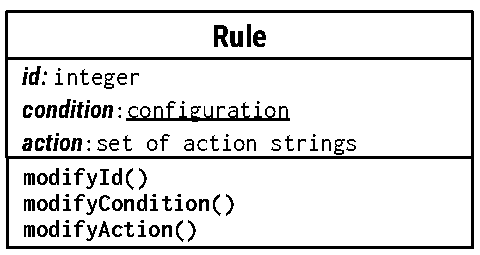
\includegraphics[scale=0.8]{figures/zzz-rule.pdf}
    \caption{Rule Class}
    \label{fig:rule}
\end{center}
\end{figure}

The \texttt{id} attribute is for rule identification. The \texttt{condition} attribute is a 
\texttt{configuration} type object. A configuration is basically a graph/network of
membranes. The \texttt{condition} attribute is a subgraph of membranes that the rule will look for
in order for it to be applicable. For example, given a reference \texttt{configuration A}, a rule is
applicable with respect to \texttt{configuration A} only if the rule's \texttt{condition}, 
\texttt{configuration B}, is a subgraph of \texttt{configuration A}. The \texttt{action} attribute
of the rule is a set of strings that specify the modifications/transformations it will perform on
a given \texttt{configuration}. e.g. The string \texttt{rc-1-3} will call
\texttt{removeConnection()} of a \texttt{configuration} to remove the connection \texttt{(1,3)}
from the \texttt{configuration}. The string \texttt{am-<id>-<lb>-1-2-3}, assuming the alphabet 
$V=\{a,b,c\}$, will call \texttt{addMembrane()} of a \texttt{configuration} to add a membrane
with \texttt{id=<id>}, \texttt{label=<lb>}, and \texttt{content=[1,2,3]} (or $a^1b^2c^3)$.

The methods \texttt{modifyId(), modifyCondition(), modifyAction()} are used to modify the attributes
of the \texttt{rule}.

% ================================================================================================ %

\item \texttt{Rule set} class simply aggregates \texttt{rules} into a set. Its only attribute is
\texttt{set} which is a set of \texttt{rules}. Methods \texttt{addARule(), removeARule(),
modifyARule()} are used to modify the \texttt{rule set}.

\begin{figure}[H]
\begin{center}
    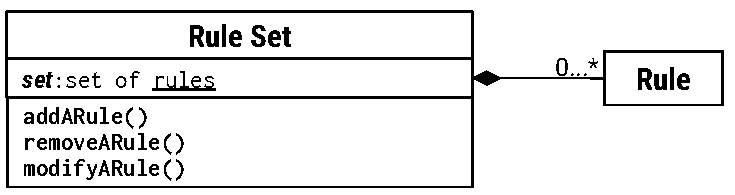
\includegraphics[scale=0.8]{figures/zzz-rule-set.pdf}
    \caption{Rule Set Class}
    \label{fig:rule-set}
\end{center}
\end{figure}

% ================================================================================================ %

\item \texttt{P system} class represents P systems (see Section \ref{s-psystem}). The class has the
following attributes: \texttt{id} (integer), \texttt{system\_configuration} 
(\texttt{configuration}), \texttt{alphabet} (set of symbols), \texttt{system\_rule\_set} 
(\texttt{rule set}), \texttt{derivation\_mode} (string).

\begin{figure}[H]
\begin{center}
    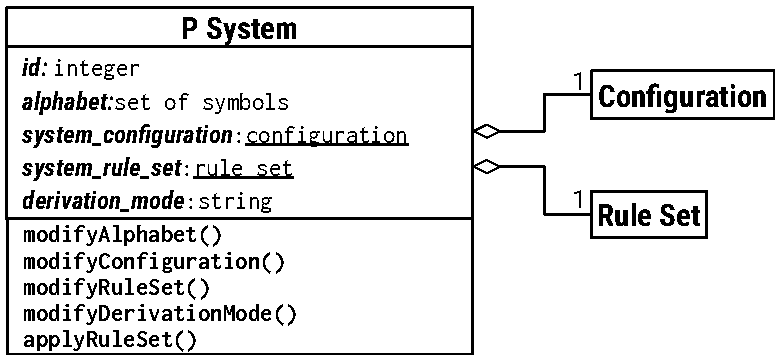
\includegraphics[scale=0.8]{figures/zzz-p-system.pdf}
    \caption{P System Class}
    \label{fig:p-system}
\end{center}
\end{figure}

The \texttt{id} attribute is for P system identification. The \texttt{alphabet} attribute is a set 
of symbols representing the types of objects in the P system. The \texttt{system\_configuration}
attribute is the initial \textit{configuration} of the P system. The \texttt{system\_rule\_set}
attribute is the set of rules of the P system. The \texttt{derivation\_mode} attribute is a string
that defines the allowable combination of rule that the P system can apply (see Section 
\ref{s-derivation}).

Methods \texttt{modifyAlphabet(), modifyConfiguration(), modifyRuleSet(), modifyDeriviationMode()}
are used to modify the attributes of the \texttt{P system}. The \texttt{applyRuleSet()} takes
allowed combination of applicable \texttt{rules} from the P system's \texttt{system\_rule\_set} and
use the \texttt{rules}' \texttt{actions} to modify the P system's \texttt{system\_configuration}.

% ================================================================================================ %

\item \texttt{Transition} class represents transitions from one \textit{configuration} to another
\textit{configuration} via application of combinations of applicable rules. The class has the
following attributes: \texttt{id} (integer), \texttt{pre\_transition\_id} (integer), 
\texttt{post\_transition\_id} (integer), \texttt{used\_rules} (set of integer).

\begin{figure}[H]
\begin{center}
    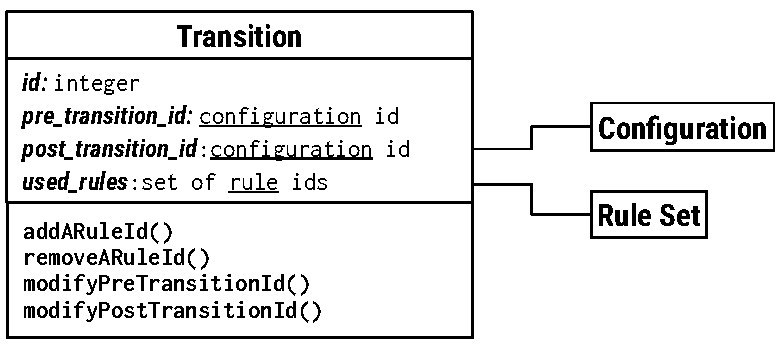
\includegraphics[scale=0.8]{figures/zzz-transition.pdf}
    \caption{Transition Class}
    \label{fig:transition-class}
\end{center}
\end{figure}

The \texttt{id} attribute is for transition identification. The \texttt{pre\_transition\_id}
attributed is an integer that is the \texttt{id} of the configuration before transition (before
rules are applied) while the \texttt{post\_transition\_id} is an integer that is the \texttt{id} of
the configuration after transition. The \texttt{used\_rules} attribute is the set of integers which
are the \texttt{ids} of the rules used in the transition.

Methods \texttt{addARuleId(), removeARuleId(), modifyPreTransitionId(), modifyPostTransitionId()}
are used to modify the attributes of the \texttt{transition}.

% ================================================================================================ %

\item \texttt{Computation} class represents the \textit{computation tree} of the P system. The
\textit{computation tree} is a tree-like network of \textit{configurations} the root of which is the
initial configuration of the P system. Starting from the root (initial) configuration, new 
configuration nodes are generated by applying allowed combinations of applicable rules to the root 
configuration then adding the resulting new configurations to the tree. Branching will occur in the
computation tree if the P system is non-deterministic such that it is possible to apply more than
one combination of rules to a given configuration. If multiple valid combinations of rules are
applied to a configuration resulting to multiple next configurations, then these are `branches' in 
the computation tree.

The class has the following attributes: \texttt{id} (integer), \texttt{configuration\_set} (set of 
\texttt{configurations}), \\ \texttt{transition\_set} (set of \texttt{transitions}).

\begin{figure}[H]
\begin{center}
    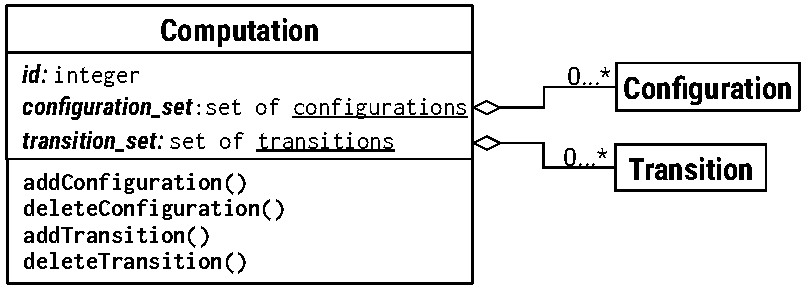
\includegraphics[scale=0.8]{figures/zzz-computation.pdf}
    \caption{Computation Class}
    \label{fig:computation-class}
\end{center}
\end{figure}

The \texttt{id} attribute is for computation identification. The \texttt{configuration\_set}
attribute is the set of \texttt{configurations} that are the nodes of the computation tree. The
\texttt{transition\_set} is the set of \texttt{transitions} between nodes of the computation tree.

Methods \texttt{addConfiguration()}, \texttt{deleteConfiguration()}, \texttt{addTransition()},
\texttt{deleteTransition()} are used to modify attributes of the \texttt{computation}.

% ================================================================================================ %

\item \texttt{PSystem-Computation} class simply combines a \texttt{P system} and its
\texttt{computation}. It has the \texttt{system} attribute for the \textit{P system} part and the
\texttt{computation} attribute for the \textit{computation} part. Methods \texttt{modifySystem()}
and \texttt{modifyComputation()} are used to modify the attributes of the
\texttt{system-computation}.

\begin{figure}[H]
\begin{center}
    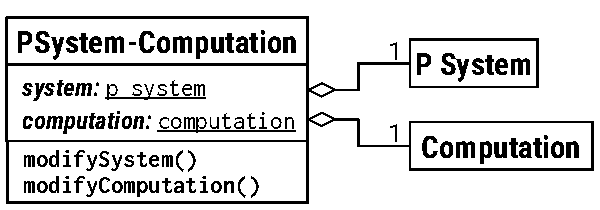
\includegraphics[scale=0.8]{figures/zzz-simulation.pdf}
    \caption{Simulation Class}
    \label{fig:simulation-class}
\end{center}
\end{figure}

% ================================================================================================ %

\end{enumerate}

% ================================================================================================ %

\subsection{User and P System Program Interactions}

The P system program's input and output is a \texttt{PSystem-Computation} object that will stored in
a file that we will call a \textit{.psy} file. The user can use two general functionalities of the P
system program: the editor functionality and the simulator functionality. As a P system editor, the
user use the P system program to open/create a $.psy$ file and edit the \texttt{P system} stored in 
the file using a graphical user interface. As a P system simulator, the user can open a $.psy$ file
and \textit{simulate} (generate the computation tree) the \texttt{P system} stored in the file.
More specific use-cases for the P system program is shown in Figure \ref{fig:use-case}.

In the following sections, the term \textit{simulation} will also refer to the computation tree or
the \texttt{computation}-type object.

\begin{figure}[H]
\begin{center}
    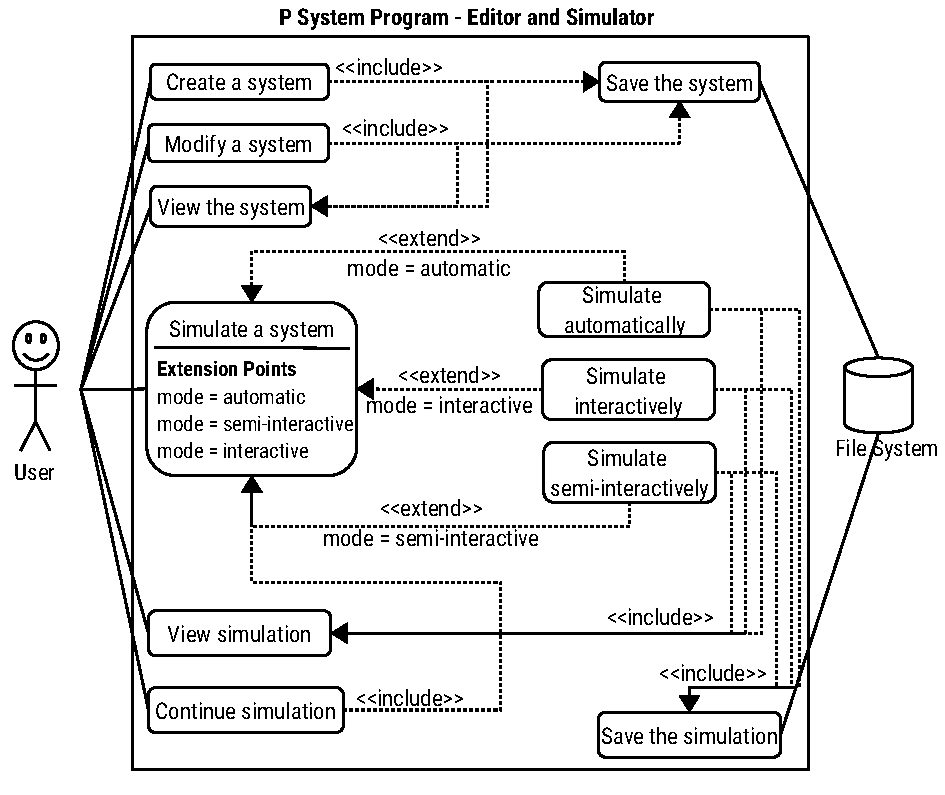
\includegraphics[scale=0.85]{figures/zzz-interaction-model.pdf}
    \caption{Use-cases for the P System Program}
    \label{fig:use-case}
\end{center}
\end{figure}

The P system program has the following six primary (user-facing) use-cases:

\begin{enumerate}
\item \texttt{Create a System:} The user can create a P system from scratch and save the system in
a \texttt{PSystem-computation} type object stored in a $.psy$ file.

\item \texttt{View a System:} The user can open an existing $.psy$ file and view the P system stored
in the file.

\item \texttt{Modify a System:} The user can open an existing $.psy$ file and modify the P system 
stored in the file. 

\item \texttt{Simulate a System:} The user can open/create a $.psy$ file then use the P system
stored in the file to generate a computation tree. The \texttt{computation} attribute of the
\texttt{PSystem-computation} object will store the simulation while the \texttt{system} attribute
will store the P system. There are 3 modes of simulation: \textit{automatic}, \textit{interactive},
and \textit{semi-interactive}. 

\begin{itemize}

\item In \texttt{mode=automatic}, the user will choose if the computation will be \textit{linear} or
\textit{branching}. The user will also specify simulation halting criteria which include the 
\textit{maximum computation depth} and \textit{maximum number of configurations}. In this mode, the
simulator part of the program will generate the configurations in the computation tree until one of
the halting criteria is met.

\item In \texttt{mode=interactive}, the simulator will generate configurations one step at a time at
user's control. If, in a given time step, there are multiple combinations of rules possible, the
user will be prompted to select one of the combinations to apply. The simulation will then proceed 
to the next configuration.

\item In \texttt{mode=semi-interactive}, the simulator will generate the configurations 
automatically as long as there are no branching involve. If there is branching in the computation, 
the user will be prompted to select one of the possible combinations of rules to apply.

\end{itemize}

After simulation the computation can then be saved in the same $.psy$ file.

\item \texttt{View Simulation:} The user can open a $.psy$ file that contains simulation/computation
of the system and view the simulation using the P system editor (GUI).

\item \texttt{Continue Simulation:} The user can open a $.psy$ file that contains computation of the
system and then continue the simulation in either of the 3 modes.

\end{enumerate}

Figure \ref{fig:gui-2} shows an example GUI for the P system program. The GUI contains the main
\textit{View Box} that shows the configuration of the P system. It has a \textit{Rules Box} that 
lists the rules of the system. It has an \textit{Add Box} that contains thing you can add to the 
P system. It has a \textit{Edit Box} that shows selected elements which can then be modified.
Figure \ref{fig:gui-2} also shows some menu options.

\begin{figure}[H]
\begin{center}
    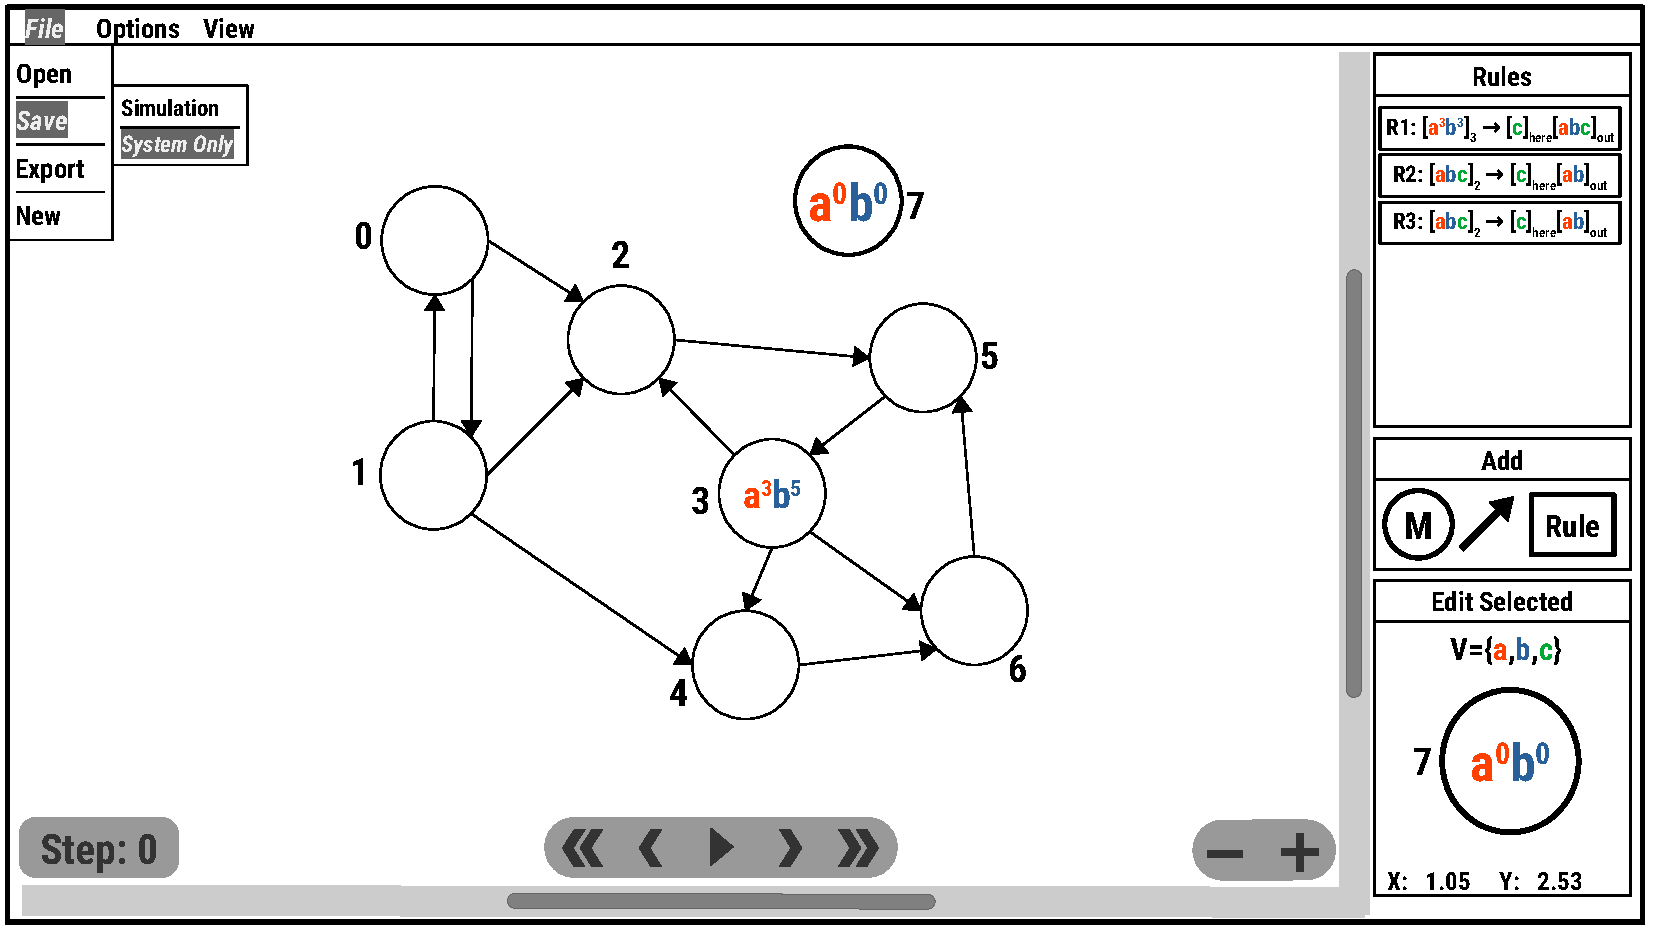
\includegraphics[scale=0.5]{figures/zzz-gui-2.pdf}
    \caption{User Interface}
    \label{fig:gui-2}
\end{center}
\end{figure}

Figure \ref{fig:gui} shows the menu option for the different simulation mode.

\begin{figure}[H]
\begin{center}
    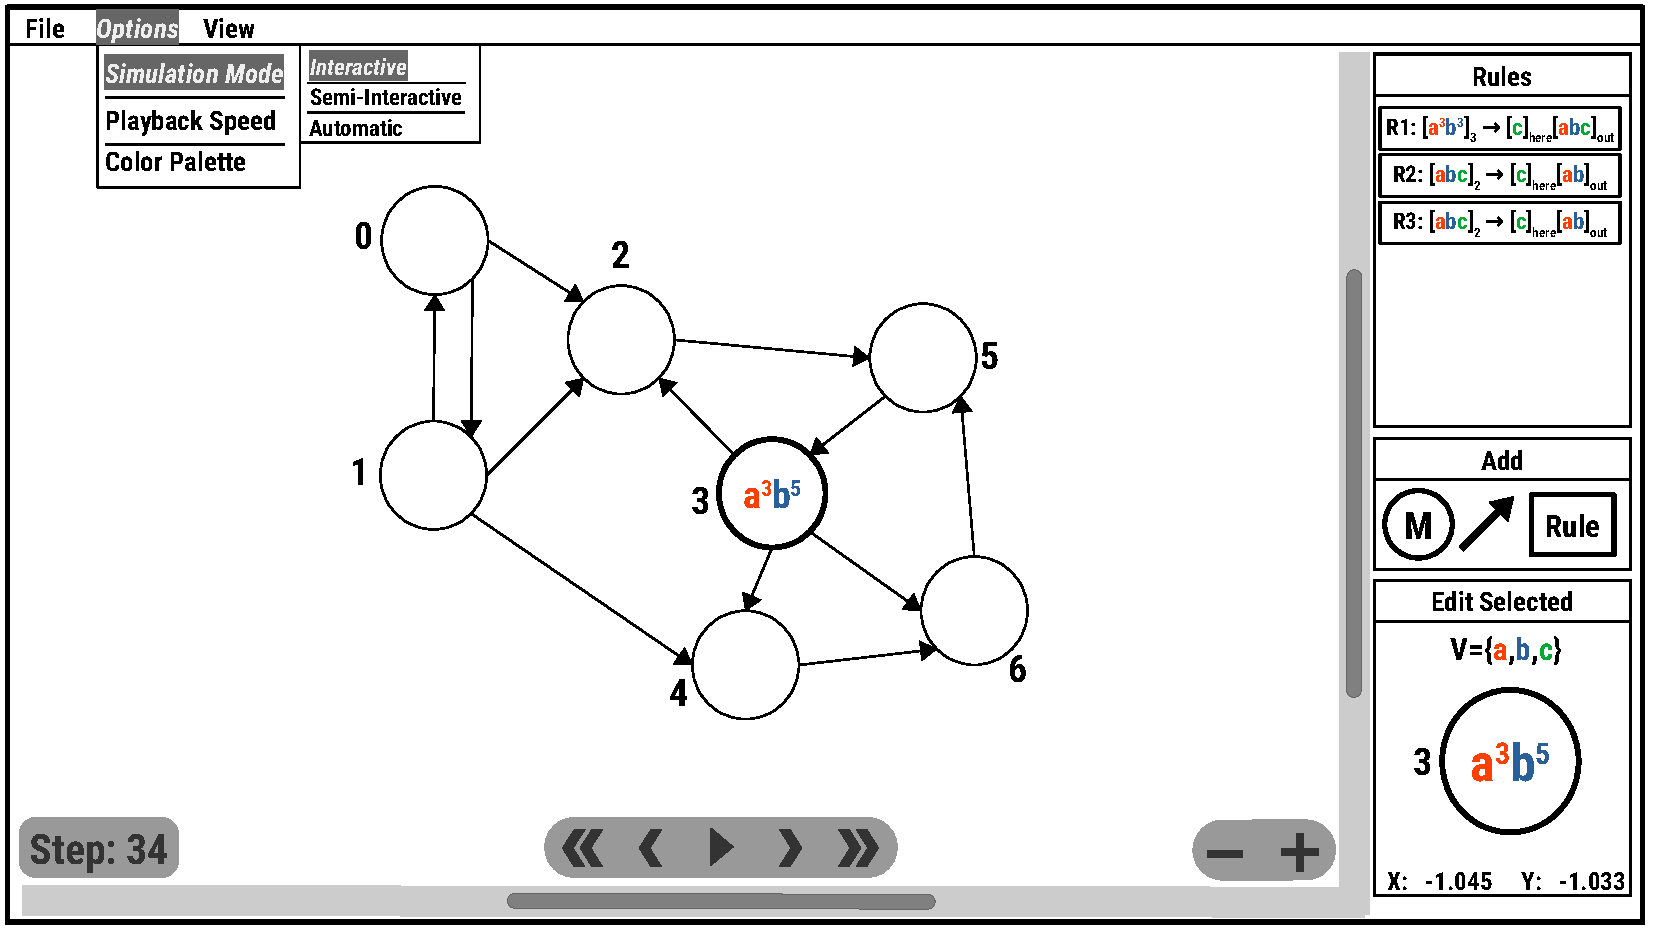
\includegraphics[scale=0.5]{figures/zzz-gui.pdf}
    \caption{User Interface}
    \label{fig:gui}
\end{center}
\end{figure}

Figure \ref{fig:gui-3} shows the \textit{computation tree} view. The \textit{view box} in the
computation tree view will show parts (some configuration) of the computation tree instead of
showing a selected configuration. A preview of the selected configuration will be shown in the
\textit{edit box}.

\begin{figure}[H]
\begin{center}
    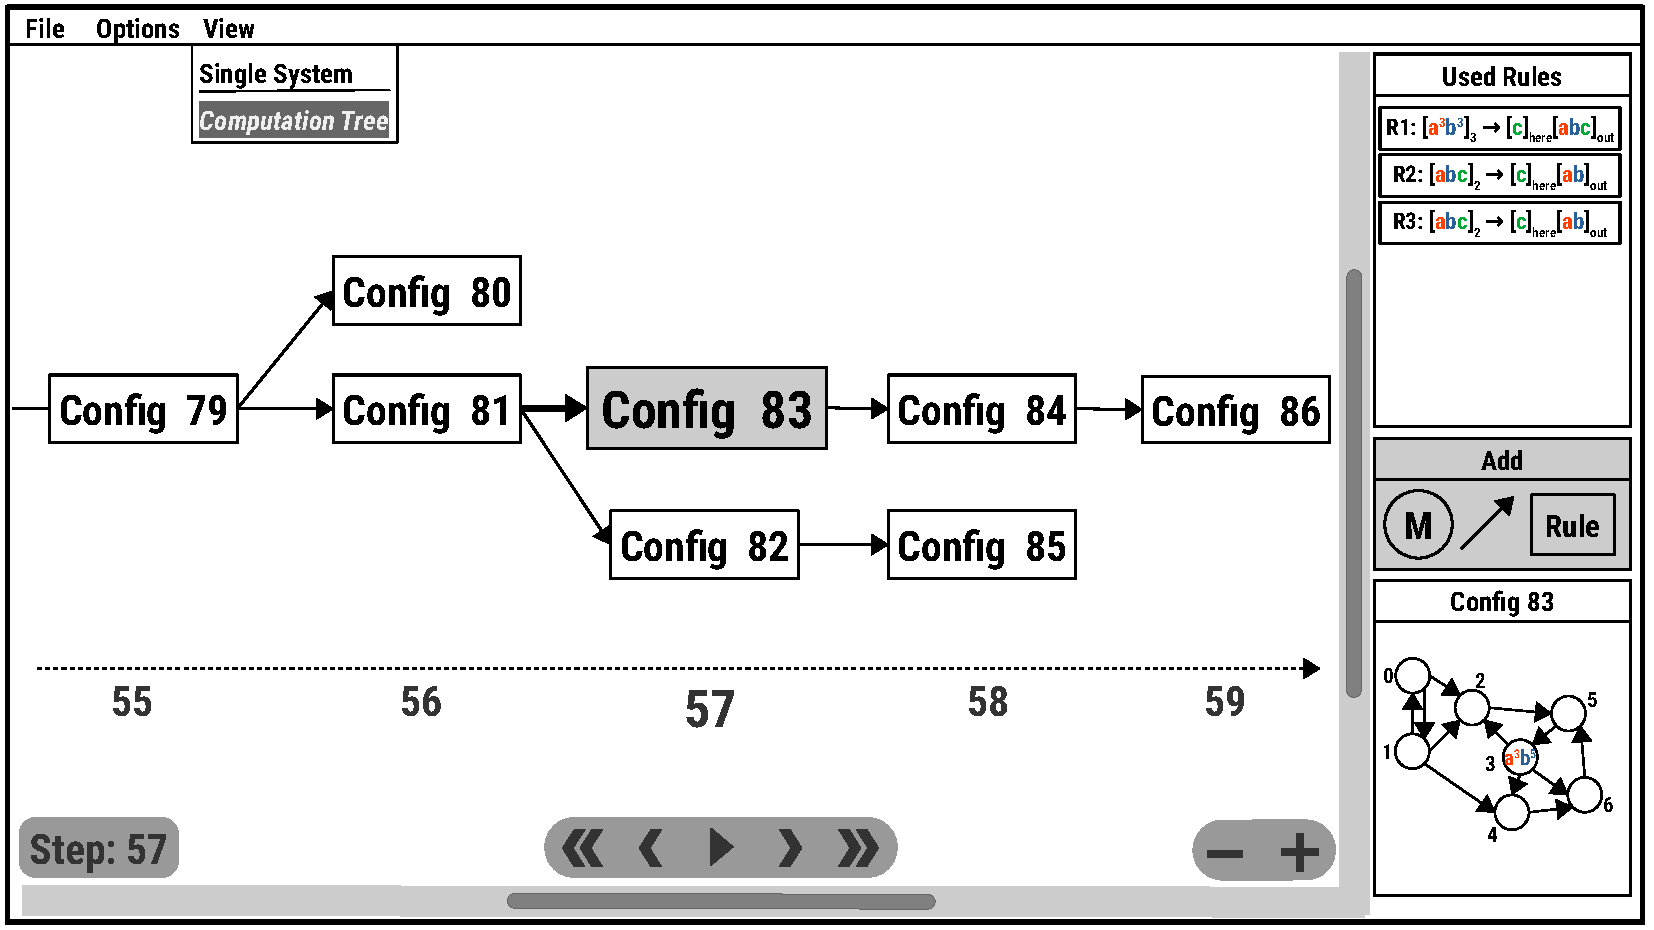
\includegraphics[scale=0.5]{figures/zzz-gui-3.pdf}
    \caption{User Interface}
    \label{fig:gui-3}
\end{center}
\end{figure}

The interface has the \texttt{(- +)} control for zooming in and out of the P system in the
\textit{single system} view. The interface also has scroll bars for changing the position of the 
\textit{view box}. The \texttt{$\langle\langle\text{   }\langle\text{  }\blacktriangleright\text{  }
\rangle\text{   }\rangle\rangle$} controls are for the simulation.

% ================================================================================================ %

\subsection{Interactions between User, P System Editor, and P System Viewer}

Figure \ref{fig:sequence-create} shows the interactions mainly between the user and the P system 
editor (GUI) for the \texttt{Create a System} use-case.

\begin{figure}[H]
\begin{center}
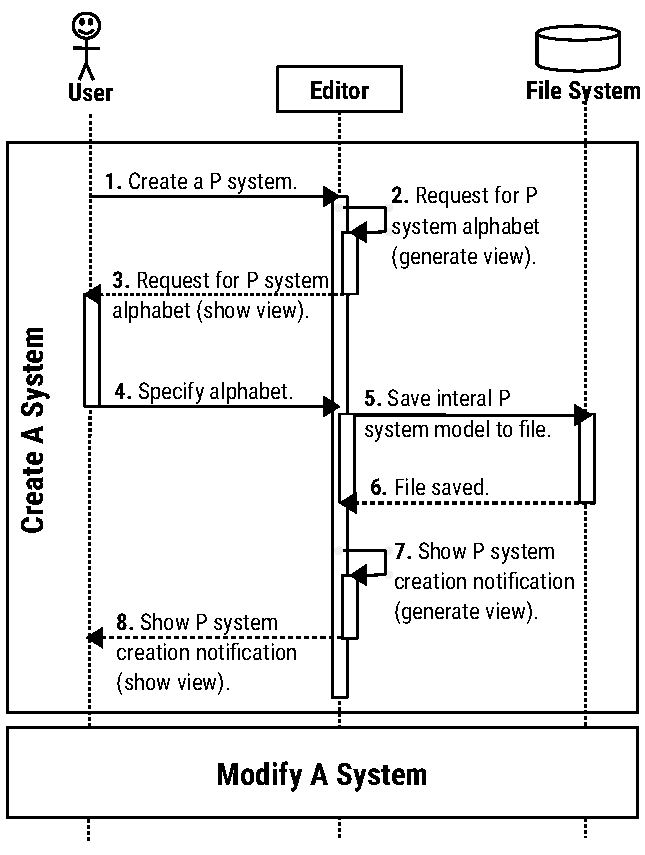
\includegraphics[scale=0.75]{figures/zzz-sequence-create.pdf}
\caption{Sequence Diagram for \texttt{Create a system} Use-case}
\label{fig:sequence-create}
\end{center}
\end{figure}

	
Creation of a new system will start with the user selecting \texttt{File > New} in the menu options 
(see Figure \ref{fig:gui-2}).  The P system editor will need to ask the user for the alphabet of 
the system. The editor will then generate an updated view (by view we mean the general interface).
The user will be prompted, by the updated view, to specify the P system's alphabet. After specifying
the alphabet the editor can now create an internal \texttt{PSystem-Computation} object and create 
the  initial template for the \texttt{system} attribute (P system) of the object. The object will 
then be stored to a $.psy$ file in the file system. The editor will generate an updated view with 
creation notification and show this view to the user.

Figure \ref{fig:sequence-modify} shows the sequence diagram for the \texttt{View a System} and 
\texttt{Modify a System} use-cases.

\begin{figure}[H]
\begin{center}
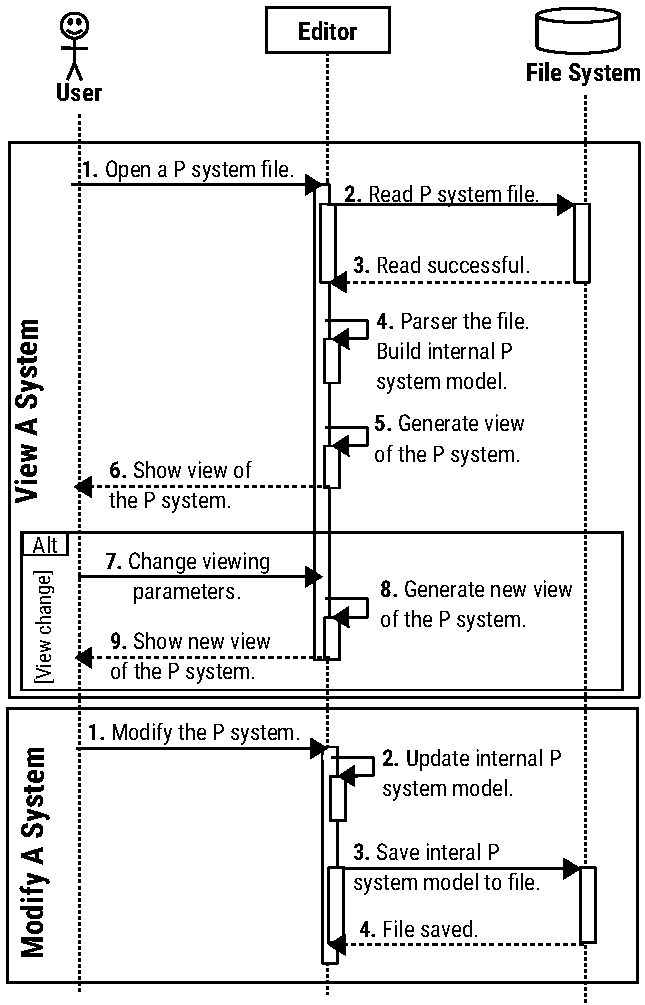
\includegraphics[scale=0.90]{figures/zzz-sequence-modify.pdf}
\caption{Sequence Diagram for \texttt{View a System} and \texttt{Modify a System} Use-cases}
\label{fig:sequence-modify}
\end{center}
\end{figure}

The user will open a $.psy$ file that contains the \texttt{PSystem-Computation} object with the
P system definition in its \texttt{system} attribute. The editor will read and parse the file then
generate the view of the P system in is \textit{view box}. The user can then view the system and
change the view box by scrolling or changing the zoom value. The user can also modify the P system
by adding component to it using controls in the \textit{add box}. If there are any changes to the
P system, the editor will update its internal copy of the P system then it will write any updates
to the $.psy$ file. \texttt{View simulation} use-case a similar sequence diagram to \texttt{View
a System} use-case. The only difference is the editor has specific procedure for parsing 
computation and has a specific procedure for generating its view.

Figure \ref{fig:sequence-simulate} shows the sequence diagram for the \texttt{Simulate a System} 
use-case.

\begin{figure}[H]
\begin{center}
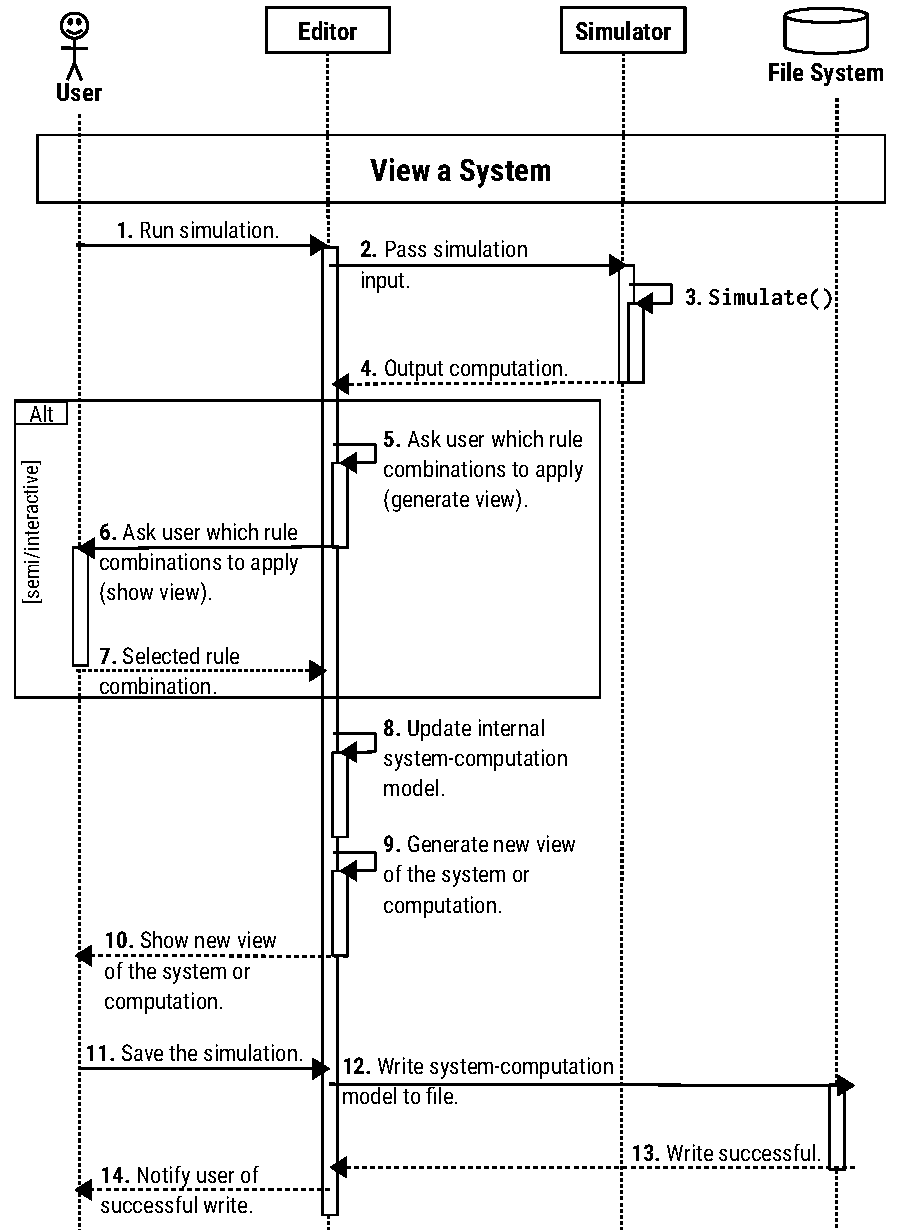
\includegraphics[scale=0.90]{figures/zzz-sequence-simulate.pdf}
\caption{Sequence Diagram for \texttt{Simulate a System} Use-case}
\label{fig:sequence-simulate}
\end{center}
\end{figure}

First, the user needs to open a $.psy$ file. The editor will use the procedure for \texttt{View a
System} use-case. The editor will then pass all simulation input to the P system simulator. The
simulation input includes the initial configuration of the system, the rule set and derivation mode
of the system, and the simulation parameters like simulation mode and halting criteria. The 
simulator will then perform the \texttt{Simulator()} procedure (to be described in Section 
\ref{s-simulate}). The \texttt{Simulator()} procedure will return an output \textit{computation}.
If the output computation contains more than one new configuration and if the mode is either
\textit{semi-interactive} or \textit{interactive}, the editor will ask the user to select which of
the valid combination of rules to apply. The editor will then update its internal copy of the
computation tree by adding the new configuration(s) and transition(s) to the tree. Then the editor
will generate a new view to reflect the changes and it will display this new view to the user.
If the user chooses to save the simulation, the internal \texttt{computation}/simulation copy of the
editor will be written to the $.psy$ file.

% ================================================================================================ %

\subsection{Internal Operations of the \texttt{Simulate()} Operation}\label{s-simulate}

\texttt{Simulate()} is the main function of the P system simulator. This function is invoked by the
P system editor if the user triggers the simulation of the system.

The \texttt{transition()} function is one of the main function used by \texttt{Simulate()}. This
function takes a \texttt{configuration}, a \texttt{rule set}, a \texttt{derivation mode}, and
simulation parameters then generate all possible valid next \texttt{configurations} and the 
\texttt{transition} objects related to each of these \texttt{configurations}. Figure 
\ref{fig:data-flow} shows the data flow diagram inside \texttt{transition()} function.

\begin{figure}[H]
\begin{center}
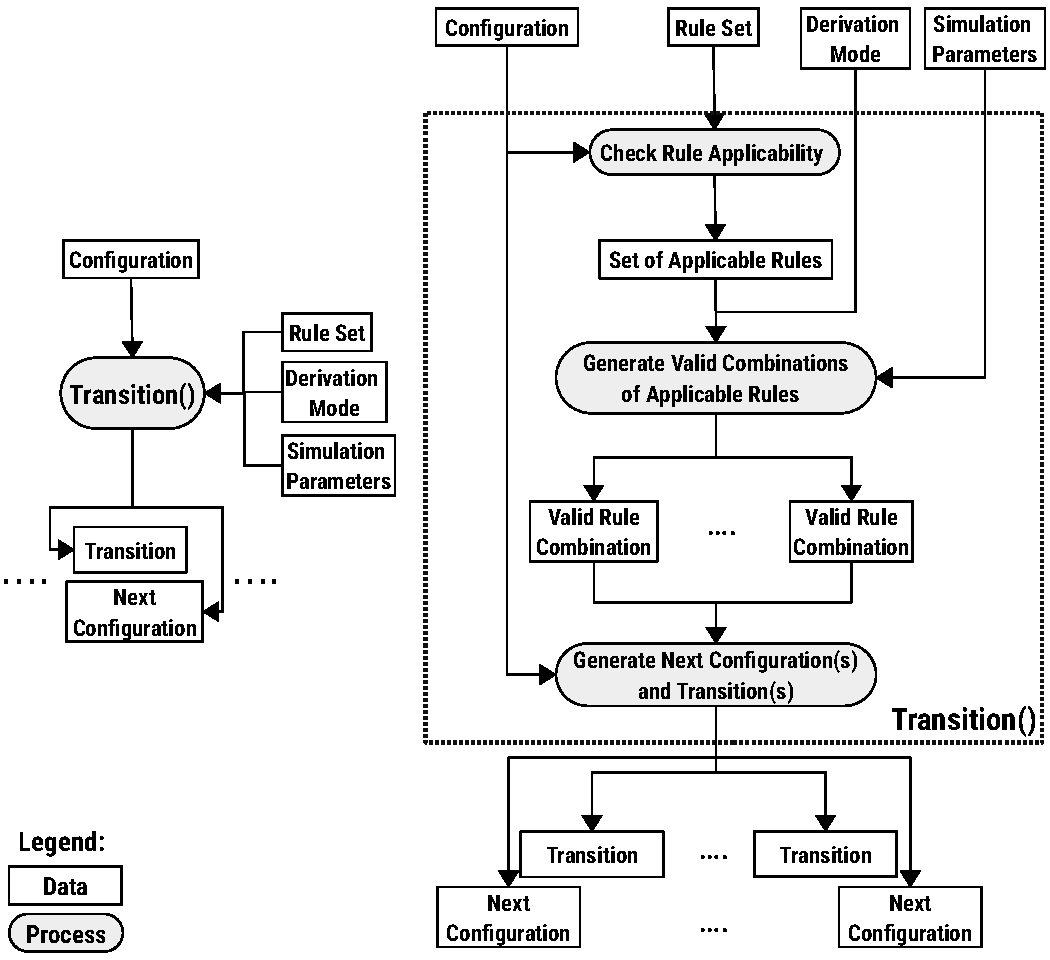
\includegraphics[scale=1]{figures/zzz-data-flow.pdf}
\caption{Data Flow of \texttt{Transition()} Operation for Generating Next Configuration(s) and 
	Transition(s)}
\label{fig:data-flow}
\end{center}
\end{figure}

\texttt{Transition()} will first check which of the rules are applicable with respect to the 
given configuration. Using the set of applicable rules, the derivation mode, and the simulation
parameters, valid combinations of applicable rules will be generated. Each valid rule combination
will be applied to the input configuration resulting to multiple next configurations and the 
transition objects for each of these new configurations.

Figure \ref{fig:data-flow-2} shows the data flow of function \texttt{Simulate()} while Figure 
\ref{fig:activity} shows \texttt{Simulate()}'s activity diagram. \texttt{Simulate()} uses 
the \texttt{Transition()} function.

\begin{figure}[H]
\begin{center}
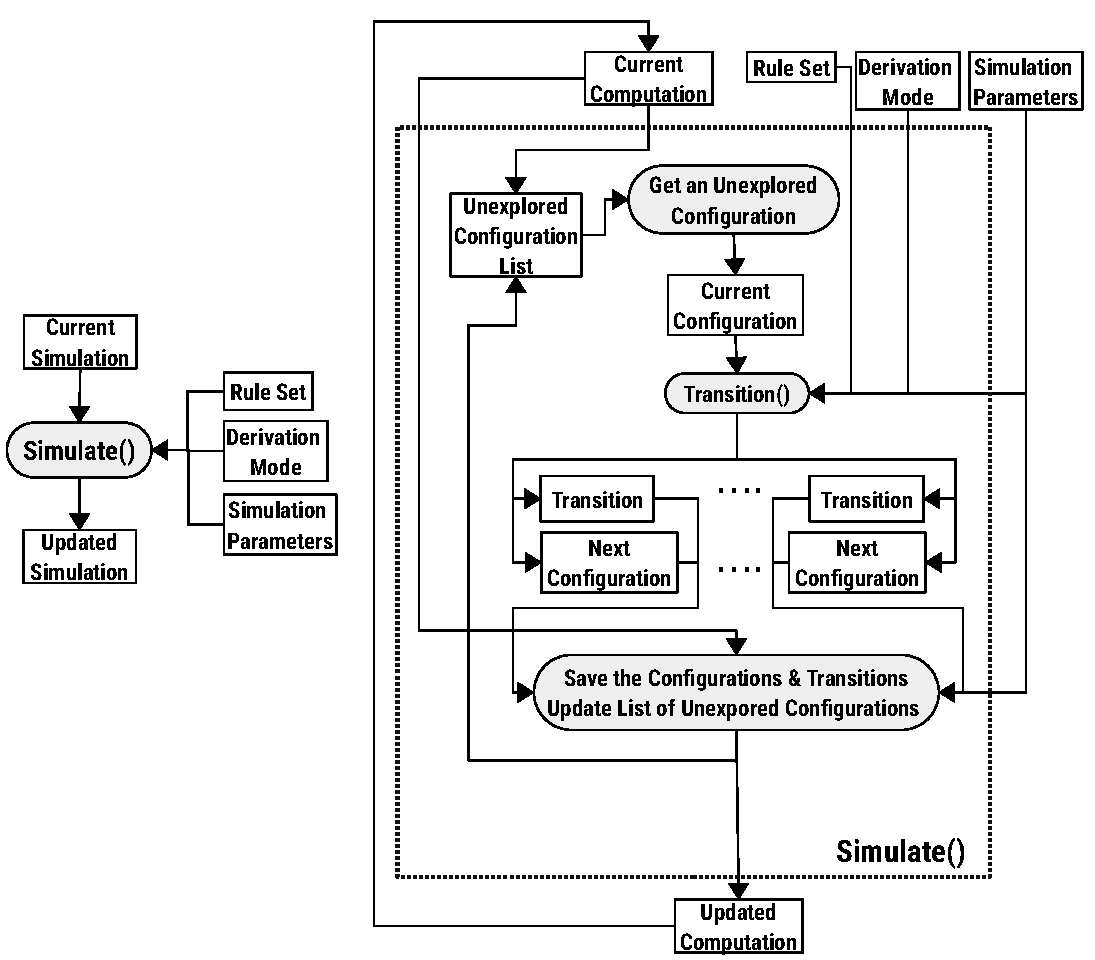
\includegraphics[scale=0.95]{figures/zzz-data-flow-2.pdf}
\caption{Data Flow of \texttt{Simulate()} Operation for Generating Updated Simulation}
\label{fig:data-flow-2}
\end{center}
\end{figure}

The input of \texttt{Simulate()} are the current computation (specifically the unexplored 
configurations of the computation tree), the P system's rule set and derivation mode, and the 
simulation parameters. All unexplored configurations from the input computation tree will be 
added to the \textit{unexplored configuration list}. The function will get the first unexplored
configuration in the list. That configuration, we will call \textit{current configuration}, will
be the input to the \texttt{Transition()} function along with the rule set, derivation mode, and
simulation parameters. The output transition(s) and next configuration(s) will be added to the
\textit{unexplored configuration list} and to the copy of the input computation. If the simulation
parameters specify a depth-first search simulation, then the new configurations will be inserted at
the beginning of the unexplored configuration list. Otherwise, if the simulation should be 
breadth-first the new configurations will be added at the back of the unexplored configuration list.
\texttt{Simulate()} will continue generating new configurations and transitions until one of the 
halt conditions, specified in the simulation parameter, is met.

\begin{figure}[H]
\begin{center}
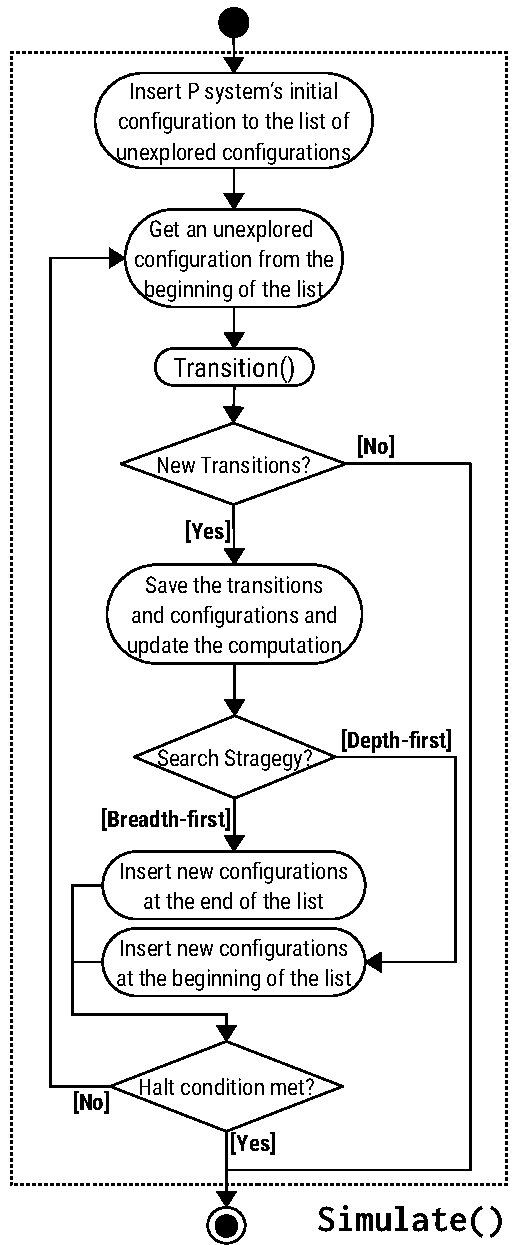
\includegraphics[scale=1]{figures/zzz-activity.pdf}
\caption{Activity Diagram for \texttt{Simulate()}}
\label{fig:activity}
\end{center}
\end{figure}

% ================================================================================================ %

\subsection{Remarks}

This design document shows a high to mid-level design for the P system program. Low-level design, 
which is very close to implementation, is not included in this document. Examples of low-level 
designs are implementation designs of procedures/functions inside \texttt{Transition()} procedure.
e.g. Checking for Rule Applicability, Generating Valid Combination of Rules, Generating Next
Configuration(s) (see Figure \ref{fig:data-flow}).

\end{document}







































